%!TEX root = ./template-skripsi.tex
%-------------------------------------------------------------------------------
% 								BAB I
% 							LATAR BELAKANG
%-------------------------------------------------------------------------------

\chapter{PENDAHULUAN}

\section{Latar Belakang Masalah}

Indonesia memiliki dua sumber perikanan: tangkap laut dan budidaya ikan air tawar. Tidak seperti memancing di laut, budidaya ikan air tawar memerlukan permodalan yang lebih besar untuk dilakukan seperti lahan, infrastruktur tambak/kolam, dan juga pakan. Hal itu belum termasuk budidaya ikan yang sulit dan memerlukan skill khusus untuk melakukannya. Namun, bukan berarti ikan hasil tangkapan laut memiliki nilai penjualan yang tinggi di setiap pasar perikanan karena adanya beberapa faktor yang mempengaruhinya seperti citarasa ikan air tawar dan ikan air laut berbeda, ikan air tawar dapat dijualbelikan dalam keadaan hidup, serta memerlukan waktu dan biaya lebih untuk menjangkau daerah-daerah tertentu seperti pegunungan untuk mengirim ikan hasil tangkapan. Dengan modal yang besar dan kemampuan khusus untuk membuat budidaya ikan air tawar, tentunya hal ini juga dapat meningkatkan potensi nilai ekonomi.

\begin{figure}[H]
	\centering
	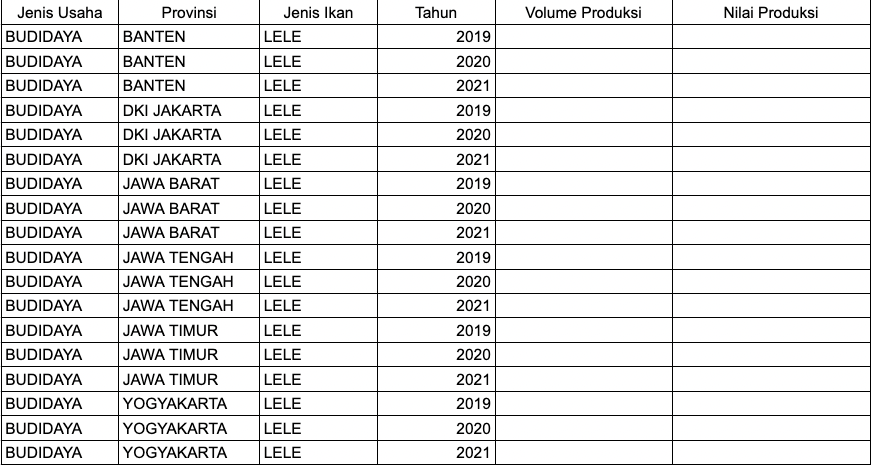
\includegraphics[keepaspectratio, width=12cm]{gambar/budidaya-ikan-lele-jawa.png}
	\caption{\emph{Produksi Ikan Lele Di Pulau Jawa} \citep{kkpdatajawa}}
	\label{gambar:budidaya-ikan-lele-jawa}
\end{figure}

\section{Rumusan Masalah}
Dari uraian latar belakang di atas, perumusan masalah pada penelitian ini ialah “Bagaimana perancangan aplikasi yang mendukung \emph{multi user} dan inventarisasi yang menjadi pendukung dalam menjalankan budidaya perikanan modern?”

\section{Pembatasan Masalah}
Pembatasan masalah pada penelitian ini antara lain:
\begin{enumerate}
	\item Aplikasi dikembangkan untuk banyak user.
	\item Pengembangan aplikasi menggunakan \emph{Framework} Flutter.
	\item Pengembangan \emph{web service} menggunakan \emph{Framework} Flask.
\end{enumerate}

\section{Tujuan Penelitian}
	Penelitian ini dilakukan dengan tujuan untuk membuat aplikasi budidaya ikan modern dengan penerapan \emph{multi user} dan inventarisasi berbasis \emph{multi platform}.

\section{Manfaat Penelitian}
\begin{enumerate}
	\item Bagi penulis
		
	Meningkatkan pengetahuan tentang teknologi budidaya perikanan modern, menambah pengalaman dalam mengembangkan aplikasi, memperoleh gelar sarjana di bidang Ilmu Komputer, serta menjadi media untuk penulis dalam mengaplikasikan ilmu yang didapat dari kampus.
		
	\item Bagi Universitas Negeri Jakarta
	 	
	Menjadi pedoman untuk penelitian di masa depan, dan dapat memberikan panduan bagi mahasiswa program studi Ilmu Komputer tentang rancang bangun aplikasi teknologi budidaya perikanan modern.
	
	\item Bagi masyarakat
	 	
	Membantu masyarakat yang ingin dan sedang menggeluti bidang budidaya perikanan dalam proses pendataan ikan dan pengelolaan lingkungan dalam budidaya itu sendiri.
	 			
\end{enumerate}


% Baris ini digunakan untuk membantu dalam melakukan sitasi
% Karena diapit dengan comment, maka baris ini akan diabaikan
% oleh compiler LaTeX.
\begin{comment}
\bibliography{daftar-pustaka}
\end{comment}
